% Options for packages loaded elsewhere
\PassOptionsToPackage{unicode}{hyperref}
\PassOptionsToPackage{hyphens}{url}
%
\documentclass[
]{article}
\usepackage{amsmath,amssymb}
\usepackage{lmodern}
\usepackage{iftex}
\ifPDFTeX
  \usepackage[T1]{fontenc}
  \usepackage[utf8]{inputenc}
  \usepackage{textcomp} % provide euro and other symbols
\else % if luatex or xetex
  \usepackage{unicode-math}
  \defaultfontfeatures{Scale=MatchLowercase}
  \defaultfontfeatures[\rmfamily]{Ligatures=TeX,Scale=1}
\fi
% Use upquote if available, for straight quotes in verbatim environments
\IfFileExists{upquote.sty}{\usepackage{upquote}}{}
\IfFileExists{microtype.sty}{% use microtype if available
  \usepackage[]{microtype}
  \UseMicrotypeSet[protrusion]{basicmath} % disable protrusion for tt fonts
}{}
\makeatletter
\@ifundefined{KOMAClassName}{% if non-KOMA class
  \IfFileExists{parskip.sty}{%
    \usepackage{parskip}
  }{% else
    \setlength{\parindent}{0pt}
    \setlength{\parskip}{6pt plus 2pt minus 1pt}}
}{% if KOMA class
  \KOMAoptions{parskip=half}}
\makeatother
\usepackage{xcolor}
\usepackage[margin=1in]{geometry}
\usepackage{color}
\usepackage{fancyvrb}
\newcommand{\VerbBar}{|}
\newcommand{\VERB}{\Verb[commandchars=\\\{\}]}
\DefineVerbatimEnvironment{Highlighting}{Verbatim}{commandchars=\\\{\}}
% Add ',fontsize=\small' for more characters per line
\usepackage{framed}
\definecolor{shadecolor}{RGB}{248,248,248}
\newenvironment{Shaded}{\begin{snugshade}}{\end{snugshade}}
\newcommand{\AlertTok}[1]{\textcolor[rgb]{0.94,0.16,0.16}{#1}}
\newcommand{\AnnotationTok}[1]{\textcolor[rgb]{0.56,0.35,0.01}{\textbf{\textit{#1}}}}
\newcommand{\AttributeTok}[1]{\textcolor[rgb]{0.77,0.63,0.00}{#1}}
\newcommand{\BaseNTok}[1]{\textcolor[rgb]{0.00,0.00,0.81}{#1}}
\newcommand{\BuiltInTok}[1]{#1}
\newcommand{\CharTok}[1]{\textcolor[rgb]{0.31,0.60,0.02}{#1}}
\newcommand{\CommentTok}[1]{\textcolor[rgb]{0.56,0.35,0.01}{\textit{#1}}}
\newcommand{\CommentVarTok}[1]{\textcolor[rgb]{0.56,0.35,0.01}{\textbf{\textit{#1}}}}
\newcommand{\ConstantTok}[1]{\textcolor[rgb]{0.00,0.00,0.00}{#1}}
\newcommand{\ControlFlowTok}[1]{\textcolor[rgb]{0.13,0.29,0.53}{\textbf{#1}}}
\newcommand{\DataTypeTok}[1]{\textcolor[rgb]{0.13,0.29,0.53}{#1}}
\newcommand{\DecValTok}[1]{\textcolor[rgb]{0.00,0.00,0.81}{#1}}
\newcommand{\DocumentationTok}[1]{\textcolor[rgb]{0.56,0.35,0.01}{\textbf{\textit{#1}}}}
\newcommand{\ErrorTok}[1]{\textcolor[rgb]{0.64,0.00,0.00}{\textbf{#1}}}
\newcommand{\ExtensionTok}[1]{#1}
\newcommand{\FloatTok}[1]{\textcolor[rgb]{0.00,0.00,0.81}{#1}}
\newcommand{\FunctionTok}[1]{\textcolor[rgb]{0.00,0.00,0.00}{#1}}
\newcommand{\ImportTok}[1]{#1}
\newcommand{\InformationTok}[1]{\textcolor[rgb]{0.56,0.35,0.01}{\textbf{\textit{#1}}}}
\newcommand{\KeywordTok}[1]{\textcolor[rgb]{0.13,0.29,0.53}{\textbf{#1}}}
\newcommand{\NormalTok}[1]{#1}
\newcommand{\OperatorTok}[1]{\textcolor[rgb]{0.81,0.36,0.00}{\textbf{#1}}}
\newcommand{\OtherTok}[1]{\textcolor[rgb]{0.56,0.35,0.01}{#1}}
\newcommand{\PreprocessorTok}[1]{\textcolor[rgb]{0.56,0.35,0.01}{\textit{#1}}}
\newcommand{\RegionMarkerTok}[1]{#1}
\newcommand{\SpecialCharTok}[1]{\textcolor[rgb]{0.00,0.00,0.00}{#1}}
\newcommand{\SpecialStringTok}[1]{\textcolor[rgb]{0.31,0.60,0.02}{#1}}
\newcommand{\StringTok}[1]{\textcolor[rgb]{0.31,0.60,0.02}{#1}}
\newcommand{\VariableTok}[1]{\textcolor[rgb]{0.00,0.00,0.00}{#1}}
\newcommand{\VerbatimStringTok}[1]{\textcolor[rgb]{0.31,0.60,0.02}{#1}}
\newcommand{\WarningTok}[1]{\textcolor[rgb]{0.56,0.35,0.01}{\textbf{\textit{#1}}}}
\usepackage{graphicx}
\makeatletter
\def\maxwidth{\ifdim\Gin@nat@width>\linewidth\linewidth\else\Gin@nat@width\fi}
\def\maxheight{\ifdim\Gin@nat@height>\textheight\textheight\else\Gin@nat@height\fi}
\makeatother
% Scale images if necessary, so that they will not overflow the page
% margins by default, and it is still possible to overwrite the defaults
% using explicit options in \includegraphics[width, height, ...]{}
\setkeys{Gin}{width=\maxwidth,height=\maxheight,keepaspectratio}
% Set default figure placement to htbp
\makeatletter
\def\fps@figure{htbp}
\makeatother
\setlength{\emergencystretch}{3em} % prevent overfull lines
\providecommand{\tightlist}{%
  \setlength{\itemsep}{0pt}\setlength{\parskip}{0pt}}
\setcounter{secnumdepth}{-\maxdimen} % remove section numbering
\ifLuaTeX
  \usepackage{selnolig}  % disable illegal ligatures
\fi
\IfFileExists{bookmark.sty}{\usepackage{bookmark}}{\usepackage{hyperref}}
\IfFileExists{xurl.sty}{\usepackage{xurl}}{} % add URL line breaks if available
\urlstyle{same} % disable monospaced font for URLs
\hypersetup{
  pdftitle={Compulsory exercise 1: Group 3},
  pdfauthor={Helle Villmones Haug, Hjalmar Jacob Vinje and Sanna Baug Warholm},
  hidelinks,
  pdfcreator={LaTeX via pandoc}}

\title{Compulsory exercise 1: Group 3}
\usepackage{etoolbox}
\makeatletter
\providecommand{\subtitle}[1]{% add subtitle to \maketitle
  \apptocmd{\@title}{\par {\large #1 \par}}{}{}
}
\makeatother
\subtitle{TMA4268 Statistical Learning V2023}
\author{Helle Villmones Haug, Hjalmar Jacob Vinje and Sanna Baug
Warholm}
\date{23 February, 2023}

\begin{document}
\maketitle

\hypertarget{problem-1}{%
\section{Problem 1}\label{problem-1}}

For this problem you will need to include some LaTex code. Please
install latex on your computer and then consult Compulsor1.Rmd for hints
how to write formulas in LaTex.

\hypertarget{a}{%
\subsection{a)}\label{a}}

We know \[
Y=f(\mathbf {x})+\varepsilon \\
\text{E}(\varepsilon)=0 \\
f(\mathbf{x}) = \mathbf{x}^T\boldsymbol{\beta}
\]

so

\[\text{E}(\widetilde{\boldsymbol \beta}) =(\mathbf{X}^\top\mathbf{X}+\lambda {\bf I})^{-1}\mathbf{X}^\top\text{E}({\bf Y}) = \\
(\mathbf{X}^\top\mathbf{X}+\lambda {\bf I})^{-1}\mathbf{X}^\top\text{E}(\mathbf{X}\beta+\epsilon) = \\
(\mathbf{X}^\top\mathbf{X}+\lambda {\bf I})^{-1}\mathbf{X}^\top\mathbf{X}\beta+0 = \\
(\mathbf{X}^\top\mathbf{X}+\lambda {\bf I})^{-1}\mathbf{X}^\top\mathbf{X}\beta \]

And the covariance matrix is then

\[\text{Cov}(\widetilde{\boldsymbol \beta}) = \text{Cov}((\mathbf{X}^\top\mathbf{X}+\lambda {\bf I})^{-1}\mathbf{X}^\top{\bf Y}) = \\
(\mathbf{X}^\top\mathbf{X}+\lambda {\bf I})^{-1}\mathbf{X}^\top \text{Cov}(\bf{Y}) ((\mathbf{X}^\top\mathbf{X}+\lambda {\bf I})^{-1}\mathbf{X}^\top)^\top
\] Cov(Y) would be only the variance:

\[
 = (\mathbf{X}^\top\mathbf{X}+\lambda {\bf I})^{-1}\mathbf{X}^\top \sigma^{2} \mathbf{I}  ((\mathbf{X}^\top\mathbf{X}+\lambda {\bf I})^{-1}\mathbf{X}^\top)^\top
\]

\hypertarget{b}{%
\subsection{b)}\label{b}}

Expected value:
\[ \text{E}(\widetilde{f}({x_0})) = \text{E}(\mathbf{x}^\top_0 \widetilde{\boldsymbol \beta}) = \mathbf{x}^\top_0 \text{E}(\widetilde{\boldsymbol \beta}) = \mathbf{x}^\top_0 (\mathbf{X}^\top\mathbf{X}+\lambda {\bf I})^{-1}\mathbf{X}^\top\mathbf{X}\beta \]
Variance:

\[ \text{Var}(\widetilde{f}({x_0})) = \text{Var}(\mathbf{x}^\top_0 \widetilde{\boldsymbol \beta}) = \mathbf{x}^\top_0 \text{Var}(\widetilde{\boldsymbol \beta}) \mathbf{x}_0 = \mathbf{x}^\top_0 (\mathbf{X}^\top\mathbf{X}+\lambda {\bf I})^{-1}\mathbf{X}^\top \text{Cov}(\bf{Y}) ((\mathbf{X}^\top\mathbf{X}+\lambda {\bf I})^{-1}\mathbf{X}^\top)^\top \mathbf{x}_0 \]
Cov(Y) would be only the variance:

\[ = \mathbf{x}^\top_0 (\mathbf{X}^\top\mathbf{X}+\lambda {\bf I})^{-1}\mathbf{X}^\top \sigma^{2} \mathbf{I} ((\mathbf{X}^\top\mathbf{X}+\lambda {\bf I})^{-1}\mathbf{X}^\top)^\top \mathbf{x}_0 \]

\hypertarget{c}{%
\subsection{c)}\label{c}}

Bias is a systematic error, in statistics it is an estimate of the
systematic difference from the true value. If a model is inflexible, it
could be underfitted and have a high bias.

Variance measures uncertainty. If variance is high, the estimate of the
distribution function is likely to change for different input data. Very
complex models might overfit data and get a high variance.

Irreducable error is the variance of a ``unknown'' variable which adds
uncorrelated noise with a mean of 0 (``random'', or unobserved
influences), which means that it cannot be reduced by improving the fit
of the model.

\hypertarget{d}{%
\subsection{d)}\label{d}}

Bias:

\[ f({x_0}) - E[\widetilde{f}({x_0})] = \mathbf{x}^\top_0 \widetilde{\boldsymbol \beta} - \mathbf{x}^\top_0 (\mathbf{X}^\top\mathbf{X}+\lambda {\bf I})^{-1}\mathbf{X}^\top\mathbf{X}\beta  \]

Variance (using previous calculations):

\[  Var(\widetilde{f}({x_0})) = \mathbf{x}^\top_0 (\mathbf{X}^\top\mathbf{X}+\lambda {\bf I})^{-1}\mathbf{X}^\top \text{Cov}(\bf{Y}) ((\mathbf{X}^\top\mathbf{X}+\lambda {\bf I})^{-1}\mathbf{X}^\top)^\top \mathbf{x}_0 \]

Irreducible error:

\[ Var(\varepsilon)= \sigma^{2} \]

MSE:

\[ MSE = \text{irreducable error + variance + squared bias} = \\ 
Var(\varepsilon) + \mathbf{x}^\top_0 (\mathbf{X}^\top\mathbf{X}+\lambda {\bf I})^{-1}\mathbf{X}^\top \text{Cov}(\bf{Y}) ((\mathbf{X}^\top\mathbf{X}+\lambda {\bf I})^{-1}\mathbf{X}^\top)^\top \mathbf{x}_0 + (\mathbf{x}^\top_0 \widetilde{\boldsymbol \beta} - \mathbf{x}^\top_0 (\mathbf{X}^\top\mathbf{X}+\lambda {\bf I})^{-1}\mathbf{X}^\top\mathbf{X}\beta)^2 \]

\hypertarget{e}{%
\subsection{e)}\label{e}}

\begin{Shaded}
\begin{Highlighting}[]
\NormalTok{id }\OtherTok{\textless{}{-}} \StringTok{"1X\_8OKcoYbng1XvYFDirxjEWr7LtpNr1m"} \CommentTok{\# google file ID}
\NormalTok{values }\OtherTok{\textless{}{-}} \FunctionTok{dget}\NormalTok{(}\FunctionTok{sprintf}\NormalTok{(}\StringTok{"https://docs.google.com/uc?id=\%s\&export=download"}\NormalTok{, id))}
\NormalTok{X }\OtherTok{\textless{}{-}}\NormalTok{ values}\SpecialCharTok{$}\NormalTok{X}
\FunctionTok{dim}\NormalTok{(X)}
\end{Highlighting}
\end{Shaded}

\begin{verbatim}
## [1] 100  81
\end{verbatim}

\begin{Shaded}
\begin{Highlighting}[]
\NormalTok{x0 }\OtherTok{\textless{}{-}}\NormalTok{ values}\SpecialCharTok{$}\NormalTok{x0}
\FunctionTok{dim}\NormalTok{(x0)}
\end{Highlighting}
\end{Shaded}

\begin{verbatim}
## [1] 81  1
\end{verbatim}

\begin{Shaded}
\begin{Highlighting}[]
\NormalTok{beta }\OtherTok{\textless{}{-}}\NormalTok{ values}\SpecialCharTok{$}\NormalTok{beta}
\FunctionTok{dim}\NormalTok{(beta)}
\end{Highlighting}
\end{Shaded}

\begin{verbatim}
## [1] 81  1
\end{verbatim}

\begin{Shaded}
\begin{Highlighting}[]
\NormalTok{sigma }\OtherTok{\textless{}{-}}\NormalTok{ values}\SpecialCharTok{$}\NormalTok{sigma}
\NormalTok{sigma}
\end{Highlighting}
\end{Shaded}

\begin{verbatim}
## [1] 0.5
\end{verbatim}

\begin{Shaded}
\begin{Highlighting}[]
\FunctionTok{library}\NormalTok{(ggplot2)}
\NormalTok{bias }\OtherTok{\textless{}{-}} \ControlFlowTok{function}\NormalTok{(lambda, X, x0, beta) \{}
\NormalTok{  p }\OtherTok{\textless{}{-}} \FunctionTok{ncol}\NormalTok{(X)}
\NormalTok{  value }\OtherTok{\textless{}{-}}\NormalTok{ (}\FunctionTok{t}\NormalTok{(x0) }\SpecialCharTok{\%*\%}\NormalTok{ beta }\SpecialCharTok{{-}} \FunctionTok{t}\NormalTok{(x0) }\SpecialCharTok{\%*\%} \FunctionTok{solve}\NormalTok{(}\FunctionTok{t}\NormalTok{(X) }\SpecialCharTok{\%*\%}\NormalTok{ X }\SpecialCharTok{+}\NormalTok{ lambda }\SpecialCharTok{*} \FunctionTok{diag}\NormalTok{(p)) }\SpecialCharTok{\%*\%} \FunctionTok{t}\NormalTok{(X) }\SpecialCharTok{\%*\%}\NormalTok{ X }\SpecialCharTok{\%*\%}\NormalTok{ beta)}\SpecialCharTok{\^{}}\DecValTok{2}
  \FunctionTok{return}\NormalTok{(value)}
\NormalTok{\}}
\NormalTok{lambdas }\OtherTok{\textless{}{-}} \FunctionTok{seq}\NormalTok{(}\DecValTok{0}\NormalTok{, }\DecValTok{2}\NormalTok{, }\AttributeTok{length.out =} \DecValTok{500}\NormalTok{)}
\NormalTok{BIAS }\OtherTok{\textless{}{-}} \FunctionTok{rep}\NormalTok{(}\ConstantTok{NA}\NormalTok{, }\FunctionTok{length}\NormalTok{(lambdas))}
\ControlFlowTok{for}\NormalTok{ (i }\ControlFlowTok{in} \FunctionTok{seq\_along}\NormalTok{(lambdas)) BIAS[i] }\OtherTok{\textless{}{-}} \FunctionTok{bias}\NormalTok{(lambdas[i], X, x0, beta)}
\NormalTok{dfBias }\OtherTok{\textless{}{-}} \FunctionTok{data.frame}\NormalTok{(}\AttributeTok{lambdas =}\NormalTok{ lambdas, }\AttributeTok{bias =}\NormalTok{ BIAS)}
\FunctionTok{ggplot}\NormalTok{(dfBias, }\FunctionTok{aes}\NormalTok{(}\AttributeTok{x =}\NormalTok{ lambdas, }\AttributeTok{y =}\NormalTok{ bias)) }\SpecialCharTok{+}
  \FunctionTok{geom\_line}\NormalTok{(}\AttributeTok{color =} \StringTok{"hotpink"}\NormalTok{) }\SpecialCharTok{+}
  \FunctionTok{xlab}\NormalTok{(}\FunctionTok{expression}\NormalTok{(lambda)) }\SpecialCharTok{+}
  \FunctionTok{ylab}\NormalTok{(}\FunctionTok{expression}\NormalTok{(bias}\SpecialCharTok{\^{}}\DecValTok{2}\NormalTok{))}
\end{Highlighting}
\end{Shaded}

\hypertarget{f}{%
\subsection{f)}\label{f}}

Now we will create the variance function which takes the same inputs as
the squared bias. As in e) you have to fill only the
\texttt{value\ \textless{}-\ ...} and run the code to plot the variance.

\begin{Shaded}
\begin{Highlighting}[]
\NormalTok{variance }\OtherTok{\textless{}{-}} \ControlFlowTok{function}\NormalTok{(lambda, X, x0, sigma) \{}
\NormalTok{  p }\OtherTok{\textless{}{-}} \FunctionTok{ncol}\NormalTok{(X)}
\NormalTok{  inv }\OtherTok{\textless{}{-}} \FunctionTok{solve}\NormalTok{(}\FunctionTok{t}\NormalTok{(X) }\SpecialCharTok{\%*\%}\NormalTok{ X }\SpecialCharTok{+}\NormalTok{ lambda }\SpecialCharTok{*} \FunctionTok{diag}\NormalTok{(p))}
\NormalTok{  value }\OtherTok{\textless{}{-}} \FunctionTok{t}\NormalTok{(x0) }\SpecialCharTok{\%*\%} \FunctionTok{solve}\NormalTok{(}\FunctionTok{t}\NormalTok{(X) }\SpecialCharTok{\%*\%}\NormalTok{ X }\SpecialCharTok{+}\NormalTok{ lambda }\SpecialCharTok{*} \FunctionTok{diag}\NormalTok{(p)) }\SpecialCharTok{\%*\%} \FunctionTok{t}\NormalTok{(X) }\SpecialCharTok{\%*\%} \FunctionTok{t}\NormalTok{(}\FunctionTok{solve}\NormalTok{(}\FunctionTok{t}\NormalTok{(X) }\SpecialCharTok{\%*\%}\NormalTok{ X }\SpecialCharTok{+}\NormalTok{ lambda }\SpecialCharTok{*} \FunctionTok{diag}\NormalTok{(p)) }\SpecialCharTok{\%*\%} \FunctionTok{t}\NormalTok{(X)) }\SpecialCharTok{\%*\%}\NormalTok{ x0 }\SpecialCharTok{*}\NormalTok{ sigma}\SpecialCharTok{\^{}}\DecValTok{2}
  \FunctionTok{return}\NormalTok{(value)}
\NormalTok{\}}
\NormalTok{lambdas }\OtherTok{\textless{}{-}} \FunctionTok{seq}\NormalTok{(}\DecValTok{0}\NormalTok{, }\DecValTok{2}\NormalTok{, }\AttributeTok{length.out =} \DecValTok{500}\NormalTok{)}
\NormalTok{VAR }\OtherTok{\textless{}{-}} \FunctionTok{rep}\NormalTok{(}\ConstantTok{NA}\NormalTok{, }\FunctionTok{length}\NormalTok{(lambdas))}
\ControlFlowTok{for}\NormalTok{ (i }\ControlFlowTok{in} \FunctionTok{seq\_along}\NormalTok{(lambdas)) VAR[i] }\OtherTok{\textless{}{-}} \FunctionTok{variance}\NormalTok{(lambdas[i], X, x0, sigma)}
\NormalTok{dfVar }\OtherTok{\textless{}{-}} \FunctionTok{data.frame}\NormalTok{(}\AttributeTok{lambdas =}\NormalTok{ lambdas, }\AttributeTok{var =}\NormalTok{ VAR)}
\FunctionTok{ggplot}\NormalTok{(dfVar, }\FunctionTok{aes}\NormalTok{(}\AttributeTok{x =}\NormalTok{ lambdas, }\AttributeTok{y =}\NormalTok{ var)) }\SpecialCharTok{+}
  \FunctionTok{geom\_line}\NormalTok{(}\AttributeTok{color =} \StringTok{"gold"}\NormalTok{) }\SpecialCharTok{+}
  \FunctionTok{xlab}\NormalTok{(}\FunctionTok{expression}\NormalTok{(lambda)) }\SpecialCharTok{+}
  \FunctionTok{ylab}\NormalTok{(}\StringTok{"variance"}\NormalTok{)}
\end{Highlighting}
\end{Shaded}

\hypertarget{g}{%
\subsection{g)}\label{g}}

Fill in the \texttt{exp\_mse} of the following code to calculate the
expected MSE for the same lambda values that you plugged in above. Then
plot all the components together and find the value of \(\lambda\) which
minimizes the expected MSE.

\begin{Shaded}
\begin{Highlighting}[]
\NormalTok{irrErr }\OtherTok{\textless{}{-}}\NormalTok{ sigma}\SpecialCharTok{\^{}}\DecValTok{2}
\NormalTok{exp\_mse }\OtherTok{\textless{}{-}}\NormalTok{ BIAS }\SpecialCharTok{+}\NormalTok{ VAR }\SpecialCharTok{+}\NormalTok{ irrErr}
\NormalTok{min\_lambda }\OtherTok{\textless{}{-}}\NormalTok{ lambdas[}\FunctionTok{which.min}\NormalTok{(exp\_mse)]}
\NormalTok{dfMSE }\OtherTok{\textless{}{-}} \FunctionTok{data.frame}\NormalTok{(}\AttributeTok{lambdas =}\NormalTok{ lambdas, }\AttributeTok{mse =}\NormalTok{ exp\_mse, }\AttributeTok{bias =}\NormalTok{ BIAS, }\AttributeTok{var =}\NormalTok{ VAR, }\AttributeTok{irrErr =}\NormalTok{ irrErr)}
\NormalTok{dfBVI }\OtherTok{\textless{}{-}} \FunctionTok{merge}\NormalTok{(dfBias, dfVar, }\AttributeTok{by =} \StringTok{"lambdas"}\NormalTok{)}

\FunctionTok{ggplot}\NormalTok{(dfMSE, }\FunctionTok{aes}\NormalTok{(}\AttributeTok{x =}\NormalTok{ lambdas)) }\SpecialCharTok{+} 
  \FunctionTok{geom\_line}\NormalTok{(}\FunctionTok{aes}\NormalTok{(}\AttributeTok{y =}\NormalTok{ bias, }\AttributeTok{color =} \StringTok{"BIAS squared"}\NormalTok{)) }\SpecialCharTok{+} 
  \FunctionTok{geom\_line}\NormalTok{(}\FunctionTok{aes}\NormalTok{(}\AttributeTok{y =}\NormalTok{ var, }\AttributeTok{color =} \StringTok{"VAR"}\NormalTok{)) }\SpecialCharTok{+} 
  \FunctionTok{geom\_line}\NormalTok{(}\FunctionTok{aes}\NormalTok{(}\AttributeTok{y =}\NormalTok{ irrErr, }\AttributeTok{color =} \StringTok{"irrErr"}\NormalTok{)) }\SpecialCharTok{+} 
  \FunctionTok{geom\_line}\NormalTok{(}\FunctionTok{aes}\NormalTok{(}\AttributeTok{y =}\NormalTok{ mse, }\AttributeTok{color =} \StringTok{"Exp. MSE"}\NormalTok{)) }\SpecialCharTok{+}
  \FunctionTok{scale\_color\_manual}\NormalTok{(}\AttributeTok{values =} \FunctionTok{c}\NormalTok{(}\StringTok{"BIAS"} \OtherTok{=} \StringTok{"blue"}\NormalTok{, }\StringTok{"VAR"} \OtherTok{=} \StringTok{"orange"}\NormalTok{, }\StringTok{"irrErr"} \OtherTok{=} \StringTok{"pink"}\NormalTok{, }\StringTok{"Exp. MSE"} \OtherTok{=} \StringTok{"purple"}\NormalTok{)) }\SpecialCharTok{+}
  \FunctionTok{xlab}\NormalTok{(}\StringTok{"lambda"}\NormalTok{) }\SpecialCharTok{+}
  \FunctionTok{ylab}\NormalTok{(}\StringTok{"Exp. MSE"}\NormalTok{) }\SpecialCharTok{+}
  \FunctionTok{ggtitle}\NormalTok{(}\FunctionTok{paste}\NormalTok{(}\StringTok{"the lambda that minimize expected MSE is "}\NormalTok{, }\FunctionTok{round}\NormalTok{(min\_lambda, }\DecValTok{3}\NormalTok{)))}
\end{Highlighting}
\end{Shaded}

\hypertarget{problem-2}{%
\section{Problem 2}\label{problem-2}}

\hypertarget{a-1}{%
\subsection{a)}\label{a-1}}

\hypertarget{i}{%
\subsubsection{i)}\label{i}}

The lm() function creates a variable to be estimatied which is
multiplied with the binary variable of rankAssocProf and rankProf. The
interpretation oof the number corresponding to the variables is that
holding all other variables constant going from a AsstProf to AssocProf
is assosiated with an increase in salary of 12,907.6 and going from
AsstProf to Prof is assosiated with an increase in salary of 45,066.0
holding all other variables constant.

\hypertarget{ii}{%
\subsubsection{ii)}\label{ii}}

To test the whole categorical variable Rank, you can use an ANOVA test
to compare the means of salary for each category of Rank.

\begin{verbatim}
             Df    Sum Sq   Mean Sq F value Pr(>F)    
rank          2 1.432e+11 7.162e+10   128.2 <2e-16 ***
Residuals   394 2.201e+11 5.586e+08                   
---
Signif. codes:  0 ‘***’ 0.001 ‘**’ 0.01 ‘*’ 0.05 ‘.’ 0.1 ‘ ’ 1
\end{verbatim}

This shows that rank as a whole has an impact on salary at the 99\%
confidence level.

\hypertarget{b-1}{%
\subsection{b)}\label{b-1}}

\begin{center}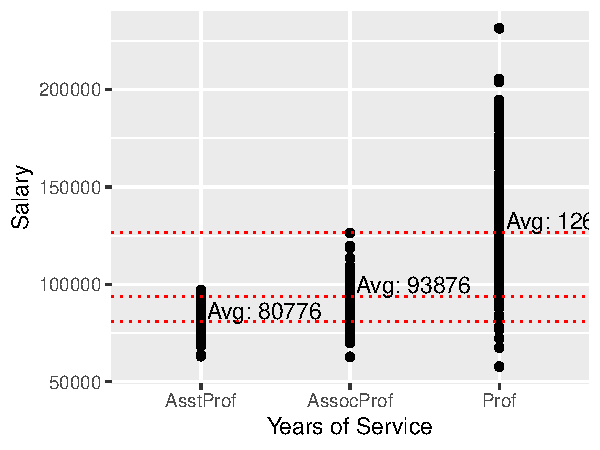
\includegraphics{Exercise1_files/figure-latex/unnamed-chunk-7-1} \end{center}

\begin{center}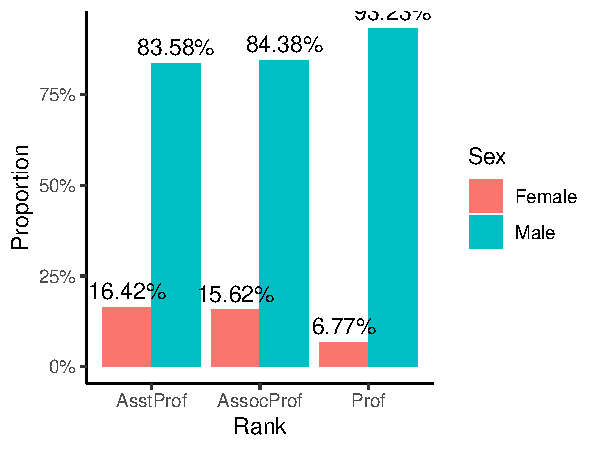
\includegraphics{Exercise1_files/figure-latex/unnamed-chunk-7-2} \end{center}

The first graph shows that professors earn more than assistante
professors and associate professors. The second shows that women make up
a higher proportion of AsstProf than Prof.

This is the reason why the regression with sex as the only covariate
shows that sex is statistically significant in trems of salary, but it
is no longer significant when controlling for rank and the other
covariates.

\hypertarget{c-1}{%
\subsection{c)}\label{c-1}}

\begin{Shaded}
\begin{Highlighting}[]
\NormalTok{model1 }\OtherTok{\textless{}{-}} \FunctionTok{lm}\NormalTok{(salary }\SpecialCharTok{\textasciitilde{}}\NormalTok{ ., }\AttributeTok{data =}\NormalTok{ Salaries)}
\FunctionTok{options}\NormalTok{(}\AttributeTok{repos =} \FunctionTok{c}\NormalTok{(}\AttributeTok{CRAN =} \StringTok{"https://cran.rstudio.com/"}\NormalTok{))}
\FunctionTok{install.packages}\NormalTok{(}\StringTok{"ggfortify"}\NormalTok{)}
\end{Highlighting}
\end{Shaded}

\begin{verbatim}
## 
## The downloaded binary packages are in
##  /var/folders/wk/x86_p6511l95p594k6qnb98h0000gn/T//RtmplJvveo/downloaded_packages
\end{verbatim}

\begin{Shaded}
\begin{Highlighting}[]
\FunctionTok{library}\NormalTok{(ggplot2)}
\FunctionTok{library}\NormalTok{(ggfortify)}
\FunctionTok{autoplot}\NormalTok{(model1, }\AttributeTok{smooth.colour =} \ConstantTok{NA}\NormalTok{)}
\end{Highlighting}
\end{Shaded}

\begin{figure}

{\centering 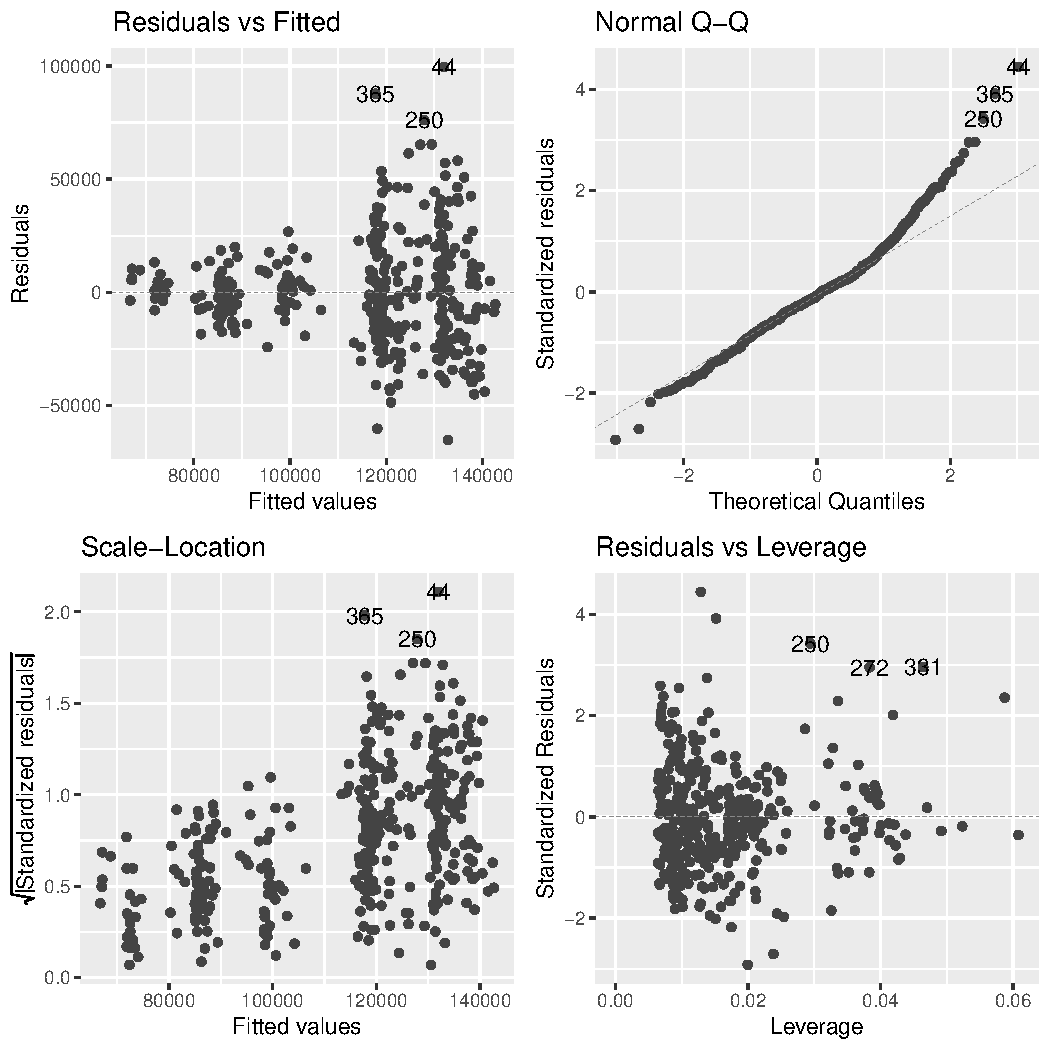
\includegraphics[width=0.7\linewidth]{Exercise1_files/figure-latex/fig_model-1} 

}

\caption{Diagnostic for model1}\label{fig:fig_model}
\end{figure}

The first plot showing residuals vs fitted values shows that the data is
heteroskedastic, meaning that the variance is not constant. This breaks
the assumption of homoscedasticity.

\hypertarget{ii-1}{%
\section{ii)}\label{ii-1}}

\begin{Shaded}
\begin{Highlighting}[]
\NormalTok{log\_salary }\OtherTok{=} \FunctionTok{log}\NormalTok{(Salaries}\SpecialCharTok{$}\NormalTok{salary)}
\NormalTok{model2 }\OtherTok{\textless{}{-}} \FunctionTok{lm}\NormalTok{(log\_salary }\SpecialCharTok{\textasciitilde{}}\NormalTok{ rank }\SpecialCharTok{+}\NormalTok{ discipline }\SpecialCharTok{+}\NormalTok{ yrs.since.phd }\SpecialCharTok{+}\NormalTok{ yrs.service }\SpecialCharTok{+}\NormalTok{ sex }\SpecialCharTok{{-}}\NormalTok{ salary, }\AttributeTok{data =}\NormalTok{ Salaries)}
\FunctionTok{library}\NormalTok{(ggplot2)}
\FunctionTok{autoplot}\NormalTok{(model2, }\AttributeTok{smooth.colour =} \ConstantTok{NA}\NormalTok{)}
\end{Highlighting}
\end{Shaded}

\begin{figure}

{\centering 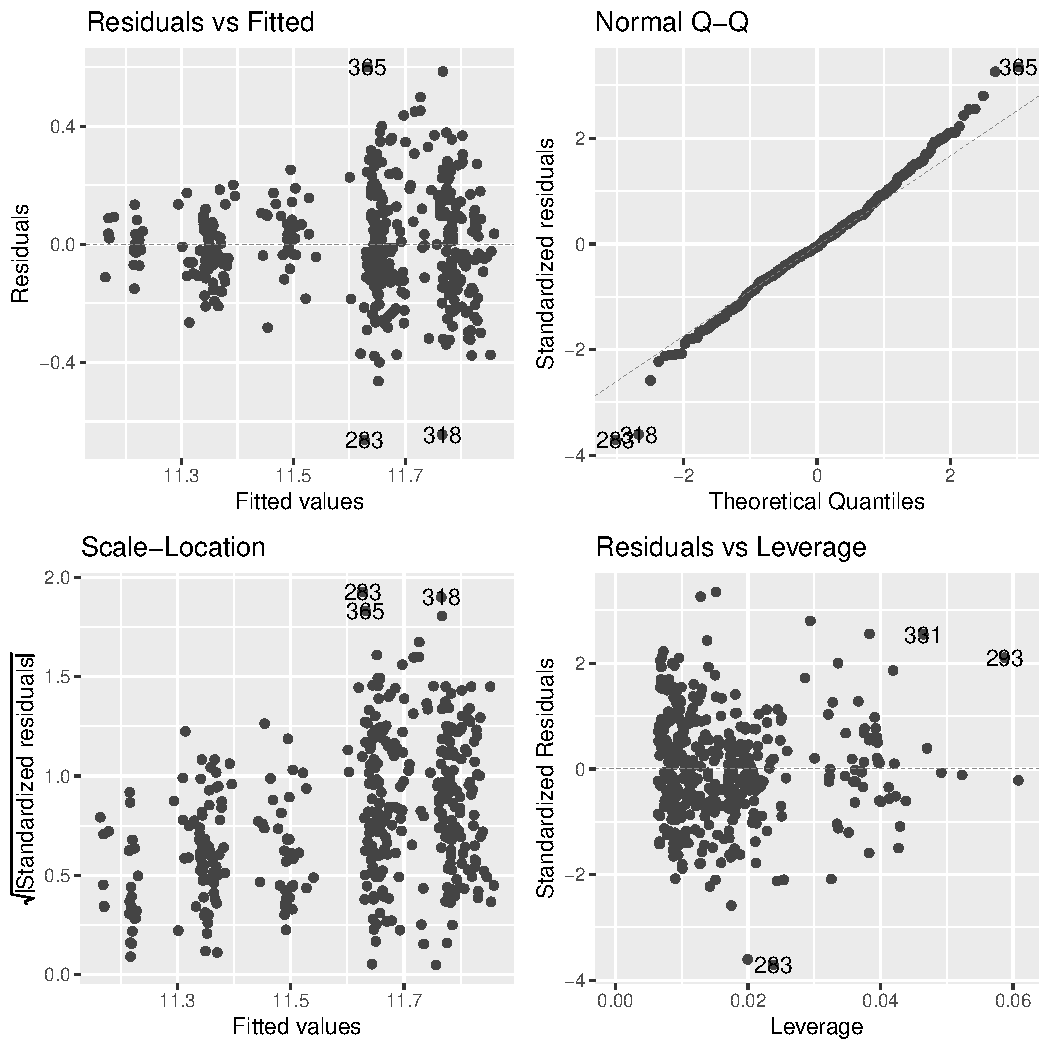
\includegraphics[width=0.7\linewidth]{Exercise1_files/figure-latex/fig_model_check-1} 

}

\caption{Diagnostic for model2}\label{fig:fig_model_check}
\end{figure}

The residual variance is still heteroskedastic.

\begin{Shaded}
\begin{Highlighting}[]
\NormalTok{log\_salary }\OtherTok{=} \FunctionTok{log}\NormalTok{(Salaries}\SpecialCharTok{$}\NormalTok{salary)}
\NormalTok{model2 }\OtherTok{\textless{}{-}} \FunctionTok{lm}\NormalTok{(log\_salary }\SpecialCharTok{\textasciitilde{}}\NormalTok{ rank }\SpecialCharTok{+}\NormalTok{ discipline }\SpecialCharTok{+}\NormalTok{ yrs.since.phd }\SpecialCharTok{+}\NormalTok{ yrs.service }\SpecialCharTok{+}\NormalTok{ sex }\SpecialCharTok{{-}}\NormalTok{ salary, }\AttributeTok{data =}\NormalTok{ Salaries)}
\FunctionTok{library}\NormalTok{(ggplot2)}
\FunctionTok{autoplot}\NormalTok{(model2, }\AttributeTok{smooth.colour =} \ConstantTok{NA}\NormalTok{)}
\end{Highlighting}
\end{Shaded}

\begin{figure}

{\centering 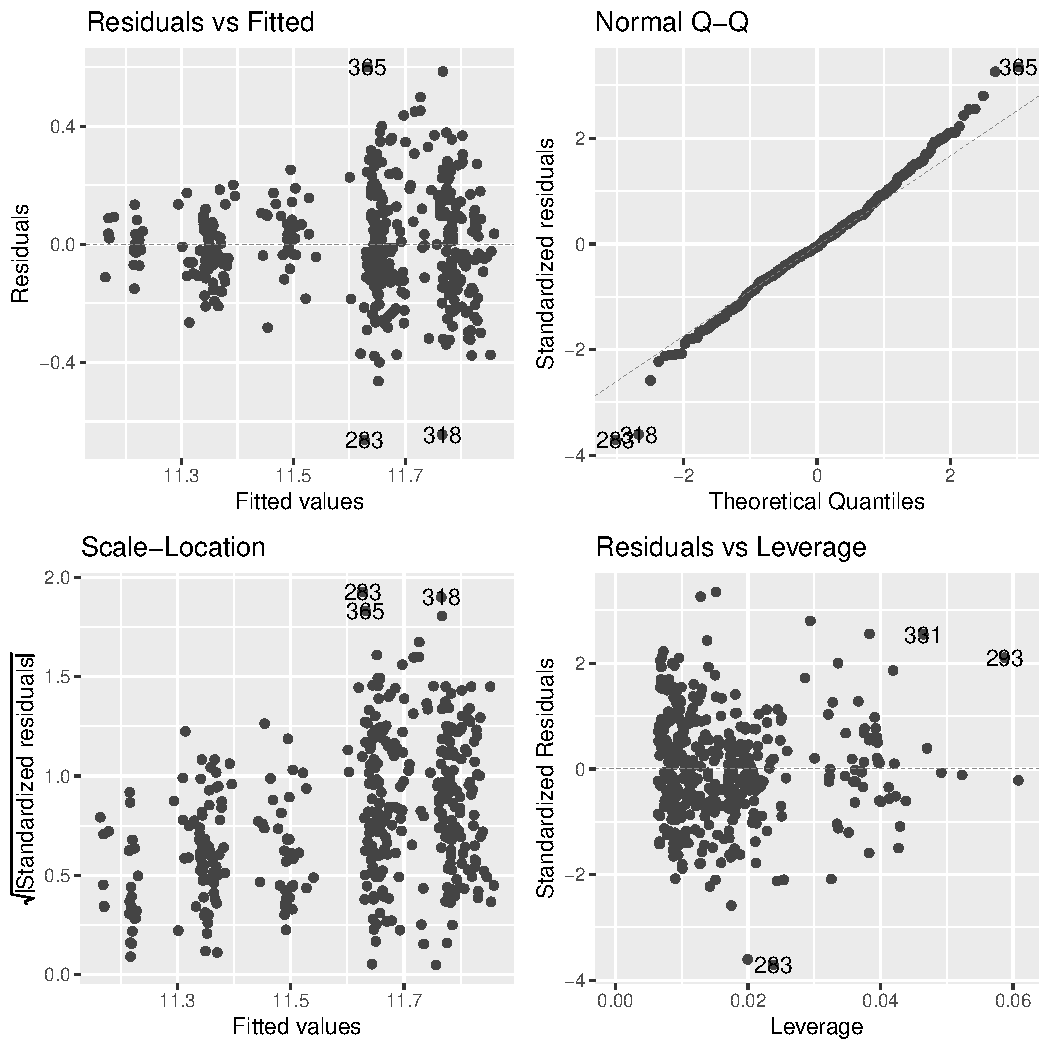
\includegraphics[width=0.7\linewidth]{Exercise1_files/figure-latex/fig_model_check_log-transform-1} 

}

\caption{Diagnostic for model3}\label{fig:fig_model_check_log-transform}
\end{figure}

\hypertarget{d-1}{%
\subsection{d)}\label{d-1}}

\begin{Shaded}
\begin{Highlighting}[]
\NormalTok{model3 }\OtherTok{\textless{}{-}} \FunctionTok{lm}\NormalTok{(log\_salary }\SpecialCharTok{\textasciitilde{}}\NormalTok{ rank }\SpecialCharTok{+}\NormalTok{ discipline }\SpecialCharTok{+}\NormalTok{ yrs.since.phd }\SpecialCharTok{+}\NormalTok{ yrs.service }\SpecialCharTok{+}\NormalTok{ sex }\SpecialCharTok{+}\NormalTok{ sex}\SpecialCharTok{:}\NormalTok{yrs.since.phd }\SpecialCharTok{{-}}\NormalTok{salary, }\AttributeTok{data =}\NormalTok{ Salaries)}
\FunctionTok{summary}\NormalTok{(model3)}
\end{Highlighting}
\end{Shaded}

\begin{verbatim}
## 
## Call:
## lm(formula = log_salary ~ rank + discipline + yrs.since.phd + 
##     yrs.service + sex + sex:yrs.since.phd - salary, data = Salaries)
## 
## Residuals:
##      Min       1Q   Median       3Q      Max 
## -0.66187 -0.10831 -0.00951  0.09846  0.60143 
## 
## Coefficients:
##                         Estimate Std. Error t value Pr(>|t|)    
## (Intercept)           11.1537511  0.0591759 188.485  < 2e-16 ***
## rankAssocProf          0.1528200  0.0335575   4.554 7.05e-06 ***
## rankProf               0.4482679  0.0344343  13.018  < 2e-16 ***
## disciplineB            0.1317818  0.0188133   7.005 1.09e-11 ***
## yrs.since.phd          0.0039500  0.0035253   1.120   0.2632    
## yrs.service           -0.0038902  0.0017059  -2.280   0.0231 *  
## sexMale                0.0574914  0.0614436   0.936   0.3500    
## yrs.since.phd:sexMale -0.0007049  0.0031407  -0.224   0.8225    
## ---
## Signif. codes:  0 '***' 0.001 '**' 0.01 '*' 0.05 '.' 0.1 ' ' 1
## 
## Residual standard error: 0.1809 on 389 degrees of freedom
## Multiple R-squared:  0.5249, Adjusted R-squared:  0.5163 
## F-statistic: 61.39 on 7 and 389 DF,  p-value: < 2.2e-16
\end{verbatim}

\begin{enumerate}
\def\labelenumi{\roman{enumi})}
\setcounter{enumi}{1}
\tightlist
\item
  The interaction term is not statistically significant, so we can not
  conclude that Bert-Ernie is correct.
\end{enumerate}

\hypertarget{e-1}{%
\subsection{e)}\label{e-1}}

\begin{Shaded}
\begin{Highlighting}[]
\CommentTok{\# i)}
\FunctionTok{set.seed}\NormalTok{(}\DecValTok{4268}\NormalTok{)}
\NormalTok{getR2 }\OtherTok{\textless{}{-}} \ControlFlowTok{function}\NormalTok{(data, indices) }
\NormalTok{  \{fit }\OtherTok{\textless{}{-}} \FunctionTok{lm}\NormalTok{(salary }\SpecialCharTok{\textasciitilde{}}\NormalTok{ rank }\SpecialCharTok{+}\NormalTok{ discipline }\SpecialCharTok{+}\NormalTok{ yrs.since.phd }\SpecialCharTok{+}\NormalTok{ yrs.service }\SpecialCharTok{+}\NormalTok{ sex,}
  \AttributeTok{data =}\NormalTok{ data[indices,])}
\FunctionTok{summary}\NormalTok{(fit)}\SpecialCharTok{$}\NormalTok{r.squared\}}
\FunctionTok{library}\NormalTok{(boot)}
\NormalTok{boot\_results }\OtherTok{\textless{}{-}} \FunctionTok{boot}\NormalTok{(}\AttributeTok{data =}\NormalTok{ Salaries, }\AttributeTok{statistic =}\NormalTok{ getR2, }\AttributeTok{R =} \DecValTok{1000}\NormalTok{, }\AttributeTok{strata =}\NormalTok{ Salaries}\SpecialCharTok{$}\NormalTok{rank)}
\end{Highlighting}
\end{Shaded}

\begin{Shaded}
\begin{Highlighting}[]
\CommentTok{\# ii)}
\FunctionTok{hist}\NormalTok{(boot\_results}\SpecialCharTok{$}\NormalTok{t, }\AttributeTok{main =} \StringTok{"Bootstrap distribution of R{-}Squared"}\NormalTok{, }
     \AttributeTok{xlab =} \StringTok{"R{-}Squared"}\NormalTok{, }\AttributeTok{col =} \StringTok{"blue"}\NormalTok{, }\AttributeTok{border =} \StringTok{"black"}\NormalTok{, }\AttributeTok{breaks =} \DecValTok{30}\NormalTok{)}
\end{Highlighting}
\end{Shaded}

\begin{center}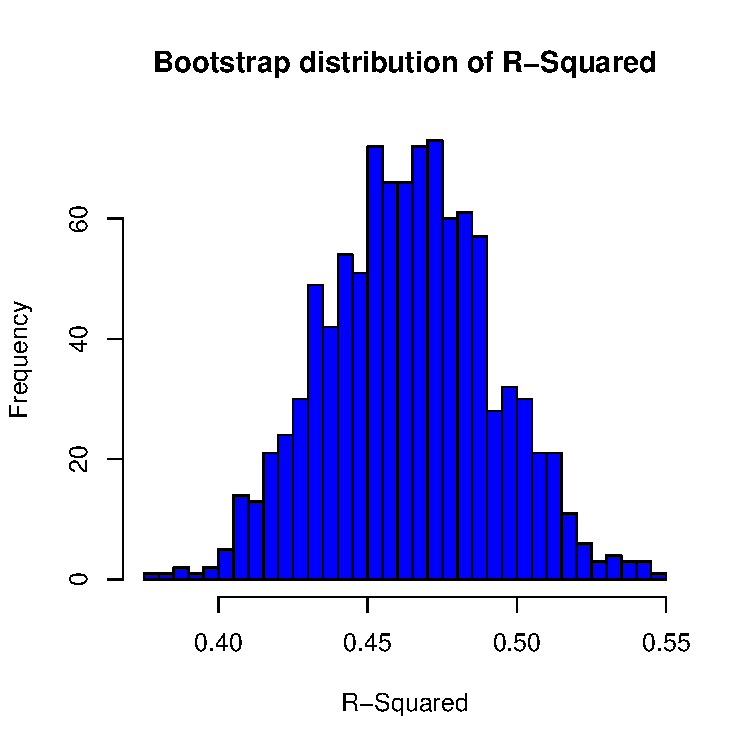
\includegraphics{Exercise1_files/figure-latex/bootstrap_plot-1} \end{center}

\begin{Shaded}
\begin{Highlighting}[]
\CommentTok{\# iii)}
\FunctionTok{sd}\NormalTok{(boot\_results}\SpecialCharTok{$}\NormalTok{t)}
\end{Highlighting}
\end{Shaded}

\begin{verbatim}
## [1] 0.02803583
\end{verbatim}

\begin{Shaded}
\begin{Highlighting}[]
\NormalTok{quant }\OtherTok{=}\NormalTok{ boot\_results}\SpecialCharTok{$}\NormalTok{t[}\DecValTok{25}\SpecialCharTok{:}\DecValTok{975}\NormalTok{]}
\FunctionTok{summary}\NormalTok{(quant)}
\end{Highlighting}
\end{Shaded}

\begin{verbatim}
##    Min. 1st Qu.  Median    Mean 3rd Qu.    Max. 
##  0.3761  0.4440  0.4644  0.4637  0.4825  0.5470
\end{verbatim}

\begin{enumerate}
\def\labelenumi{(\roman{enumi})}
\setcounter{enumi}{3}
\tightlist
\item
  R-squared was calculated to 0.5249 and the bootstrap estimates
  0.4546766 with a 95\% confidence interval of {[}0.3761, 0.5470{]}.The
  original R-squared lies within the 95\% confidence interval.
\end{enumerate}

\hypertarget{f-1}{%
\subsection{f)}\label{f-1}}

\begin{Shaded}
\begin{Highlighting}[]
\CommentTok{\# i)}
\NormalTok{bert\_ernie }\OtherTok{\textless{}{-}} \FunctionTok{data.frame}\NormalTok{(}\AttributeTok{rank=}\FunctionTok{c}\NormalTok{(}\StringTok{"Prof"}\NormalTok{, }\StringTok{"Prof"}\NormalTok{), }\AttributeTok{discipline=}\FunctionTok{c}\NormalTok{(}\StringTok{"A"}\NormalTok{, }\StringTok{"B"}\NormalTok{), }
                         \AttributeTok{yrs.since.phd=}\FunctionTok{c}\NormalTok{(}\DecValTok{20}\NormalTok{, }\DecValTok{20}\NormalTok{), }\AttributeTok{yrs.service=}\FunctionTok{c}\NormalTok{(}\DecValTok{20}\NormalTok{, }\DecValTok{20}\NormalTok{), }
                         \AttributeTok{sex=}\FunctionTok{c}\NormalTok{(}\StringTok{"Male"}\NormalTok{, }\StringTok{"Male"}\NormalTok{))}
\NormalTok{preds }\OtherTok{\textless{}{-}} \FunctionTok{predict}\NormalTok{(}\AttributeTok{object=}\NormalTok{model1, }\AttributeTok{newdata=}\NormalTok{bert\_ernie, }\AttributeTok{interval=}\StringTok{"prediction"}\NormalTok{, }\AttributeTok{level=}\FloatTok{0.95}\NormalTok{) }
\CommentTok{\# 1. Corrected confidence to prediction}
\CommentTok{\# 2. Corrected 0.975 to 0.95}
\NormalTok{preds[}\DecValTok{1}\NormalTok{, }\DecValTok{2}\NormalTok{] }\SpecialCharTok{\textgreater{}} \DecValTok{75000}
\end{Highlighting}
\end{Shaded}

\begin{verbatim}
## [1] FALSE
\end{verbatim}

He can now no longer be confident with 95\% certainty that we will earn
at least \$75 000 at this time.

\begin{enumerate}
\def\labelenumi{\roman{enumi})}
\setcounter{enumi}{1}
\tightlist
\item
  The analytic expression for the lower limit of the prediction
  interval: \[
  PI_{lower} = \boldsymbol{x}_0^T \hat{\boldsymbol{\beta}} - t_{n-p} (1-\alpha/2) \hat{\sigma} \sqrt{1+ \boldsymbol{x}_0^T (X^TX)^{-1} \boldsymbol{x}_0}
  \]
\end{enumerate}

\begin{Shaded}
\begin{Highlighting}[]
\NormalTok{x\_0 }\OtherTok{=} \FunctionTok{c}\NormalTok{(}\DecValTok{1}\NormalTok{, }\DecValTok{0}\NormalTok{, }\DecValTok{1}\NormalTok{, }\DecValTok{0}\NormalTok{, }\DecValTok{20}\NormalTok{, }\DecValTok{20}\NormalTok{, }\DecValTok{1}\NormalTok{)}
\NormalTok{beta\_hat }\OtherTok{=} \FunctionTok{coef}\NormalTok{(model1)}
\NormalTok{alpha }\OtherTok{=} \FloatTok{0.05}
\NormalTok{sd\_hat }\OtherTok{=} \FunctionTok{summary}\NormalTok{(model1)}\SpecialCharTok{$}\NormalTok{sigma}
\NormalTok{X }\OtherTok{\textless{}{-}} \FunctionTok{model.matrix}\NormalTok{(}\SpecialCharTok{\textasciitilde{}}\NormalTok{rank}\SpecialCharTok{+}\NormalTok{discipline}\SpecialCharTok{+}\NormalTok{yrs.since.phd}\SpecialCharTok{+}\NormalTok{yrs.service}\SpecialCharTok{+}\NormalTok{sex, }\AttributeTok{data=}\NormalTok{Salaries)}
\NormalTok{n }\OtherTok{=} \FunctionTok{nrow}\NormalTok{(Salaries)}
\NormalTok{p }\OtherTok{=} \FunctionTok{ncol}\NormalTok{(X)}
\NormalTok{PI\_lower }\OtherTok{=} \FunctionTok{t}\NormalTok{(x\_0)}\SpecialCharTok{\%*\%}\NormalTok{beta\_hat }\SpecialCharTok{{-}} \FunctionTok{qt}\NormalTok{(}\DecValTok{1}\SpecialCharTok{{-}}\NormalTok{alpha}\SpecialCharTok{/}\DecValTok{2}\NormalTok{,}\AttributeTok{df=}\NormalTok{n}\SpecialCharTok{{-}}\NormalTok{p) }\SpecialCharTok{*}\NormalTok{ sd\_hat }\SpecialCharTok{*} 
  \FunctionTok{sqrt}\NormalTok{(}\DecValTok{1}\SpecialCharTok{+}\FunctionTok{t}\NormalTok{(x\_0)}\SpecialCharTok{\%*\%}\FunctionTok{solve}\NormalTok{(}\FunctionTok{t}\NormalTok{(X)}\SpecialCharTok{\%*\%}\NormalTok{X)}\SpecialCharTok{\%*\%}\NormalTok{x\_0)}
\NormalTok{PI\_lower}
\end{Highlighting}
\end{Shaded}

\begin{verbatim}
##          [,1]
## [1,] 72121.12
\end{verbatim}

\begin{Shaded}
\begin{Highlighting}[]
\NormalTok{PI\_lower }\SpecialCharTok{==}\NormalTok{ preds[}\DecValTok{1}\NormalTok{,}\DecValTok{2}\NormalTok{]}
\end{Highlighting}
\end{Shaded}

\begin{verbatim}
##      [,1]
## [1,] TRUE
\end{verbatim}

\hypertarget{problem-3}{%
\section{Problem 3}\label{problem-3}}

\hypertarget{the-bigfoot-field-researchers-organization-bfro-problem-using-the-suggested-code}{%
\section{The Bigfoot Field Researchers Organization (BFRO)-problem,
using the suggested
code}\label{the-bigfoot-field-researchers-organization-bfro-problem-using-the-suggested-code}}

\begin{Shaded}
\begin{Highlighting}[]
\NormalTok{bigfoot\_original }\OtherTok{\textless{}{-}}\NormalTok{ readr}\SpecialCharTok{::}\FunctionTok{read\_csv}\NormalTok{(}\StringTok{"https://raw.githubusercontent.com/rfordatascience/tidytuesday/master/data/2022/2022{-}09{-}13/bigfoot.csv"}\NormalTok{)}
\end{Highlighting}
\end{Shaded}

Plus the data preparation, not included in the pdf (but shown in the
Rmarkdown-file)

Next, setting seed and creating training- and test-sets:

\begin{Shaded}
\begin{Highlighting}[]
\FunctionTok{set.seed}\NormalTok{(}\DecValTok{2023}\NormalTok{)}
\CommentTok{\# 70\% of the sample size for training set}
\NormalTok{training\_set\_size }\OtherTok{\textless{}{-}} \FunctionTok{floor}\NormalTok{(}\FloatTok{0.7} \SpecialCharTok{*} \FunctionTok{nrow}\NormalTok{(bigfoot))}
\NormalTok{train\_ind }\OtherTok{\textless{}{-}} \FunctionTok{sample}\NormalTok{(}\FunctionTok{seq\_len}\NormalTok{(}\FunctionTok{nrow}\NormalTok{(bigfoot)), }\AttributeTok{size =}\NormalTok{ training\_set\_size)}
\NormalTok{train }\OtherTok{\textless{}{-}}\NormalTok{ bigfoot[train\_ind, ]}
\NormalTok{test }\OtherTok{\textless{}{-}}\NormalTok{ bigfoot[}\SpecialCharTok{{-}}\NormalTok{train\_ind, ]}
\end{Highlighting}
\end{Shaded}

\hypertarget{task-a}{%
\subsection{Task a)}\label{task-a}}

\hypertarget{i-1}{%
\subsubsection{(i)}\label{i-1}}

\begin{Shaded}
\begin{Highlighting}[]
\NormalTok{model }\OtherTok{\textless{}{-}} \FunctionTok{glm}\NormalTok{(class}\SpecialCharTok{\textasciitilde{}}\NormalTok{longitude}\SpecialCharTok{+}\NormalTok{latitude}\SpecialCharTok{+}\NormalTok{visibility}\SpecialCharTok{+}\NormalTok{fur}\SpecialCharTok{+}\NormalTok{howl}\SpecialCharTok{+}\NormalTok{saw}\SpecialCharTok{+}\NormalTok{heard, }\AttributeTok{family=}\StringTok{"binomial"}\NormalTok{, }\AttributeTok{data=}\NormalTok{train)}

\NormalTok{glm\_probabilities }\OtherTok{\textless{}{-}} \FunctionTok{predict}\NormalTok{(model, test, }\AttributeTok{type=}\StringTok{"response"}\NormalTok{)}
\NormalTok{no\_classified }\OtherTok{=} \FunctionTok{sum}\NormalTok{(glm\_probabilities }\SpecialCharTok{\textgreater{}=} \FloatTok{0.5}\NormalTok{)}
\NormalTok{no\_classified }\CommentTok{\# Number of reports classified as clear sightings: 441}
\end{Highlighting}
\end{Shaded}

\begin{verbatim}
## [1] 441
\end{verbatim}

Number of clear sightings: 441

\hypertarget{ii-2}{%
\subsubsection{(ii)}\label{ii-2}}

\begin{Shaded}
\begin{Highlighting}[]
\FunctionTok{summary}\NormalTok{(model)}
\end{Highlighting}
\end{Shaded}

\begin{verbatim}
## 
## Call:
## glm(formula = class ~ longitude + latitude + visibility + fur + 
##     howl + saw + heard, family = "binomial", data = train)
## 
## Deviance Residuals: 
##     Min       1Q   Median       3Q      Max  
## -2.0710  -1.0149  -0.4291   1.0007   2.1469  
## 
## Coefficients:
##              Estimate Std. Error z value Pr(>|z|)    
## (Intercept)  0.989051   0.422048   2.343 0.019106 *  
## longitude   -0.003112   0.003460  -0.900 0.368374    
## latitude    -0.036988   0.009849  -3.756 0.000173 ***
## visibility  -0.005681   0.023686  -0.240 0.810449    
## furTRUE      0.575172   0.136328   4.219 2.45e-05 ***
## howlTRUE    -0.792152   0.189803  -4.174 3.00e-05 ***
## sawTRUE      1.291894   0.097630  13.233  < 2e-16 ***
## heardTRUE   -1.075540   0.099634 -10.795  < 2e-16 ***
## ---
## Signif. codes:  0 '***' 0.001 '**' 0.01 '*' 0.05 '.' 0.1 ' ' 1
## 
## (Dispersion parameter for binomial family taken to be 1)
## 
##     Null deviance: 2948.6  on 2126  degrees of freedom
## Residual deviance: 2509.9  on 2119  degrees of freedom
## AIC: 2525.9
## 
## Number of Fisher Scoring iterations: 4
\end{verbatim}

The coefficients for sawTRUE is 1.29, which means that the average
change in log odds with one unit increase of the value.

\begin{Shaded}
\begin{Highlighting}[]
\NormalTok{change }\OtherTok{\textless{}{-}} \FunctionTok{exp}\NormalTok{(}\FloatTok{1.29}\NormalTok{)}
\FunctionTok{print}\NormalTok{(change)}
\end{Highlighting}
\end{Shaded}

\begin{verbatim}
## [1] 3.632787
\end{verbatim}

The answer is therefore D) Multiply by 3.64'')

\hypertarget{task-b}{%
\subsection{Task b)}\label{task-b}}

\hypertarget{i-2}{%
\subsubsection{(i)}\label{i-2}}

\begin{Shaded}
\begin{Highlighting}[]
\FunctionTok{require}\NormalTok{(MASS)}
\NormalTok{qda\_model }\OtherTok{\textless{}{-}} \FunctionTok{qda}\NormalTok{(class}\SpecialCharTok{\textasciitilde{}}\NormalTok{longitude}\SpecialCharTok{+}\NormalTok{latitude}\SpecialCharTok{+}\NormalTok{visibility}\SpecialCharTok{+}\NormalTok{fur}\SpecialCharTok{+}\NormalTok{howl}\SpecialCharTok{+}\NormalTok{saw}\SpecialCharTok{+}\NormalTok{heard, }\AttributeTok{data=}\NormalTok{train)}
\NormalTok{qda\_predicted }\OtherTok{\textless{}{-}} \FunctionTok{predict}\NormalTok{(qda\_model, test)}
\FunctionTok{table}\NormalTok{(qda\_predicted}\SpecialCharTok{$}\NormalTok{class) }
\end{Highlighting}
\end{Shaded}

\begin{verbatim}
## 
##   0   1 
## 286 626
\end{verbatim}

Number of clear sightings: 626

\hypertarget{ii-3}{%
\subsubsection{(ii)}\label{ii-3}}

1): True, 2): False, 3): False, 4): False

\hypertarget{task-c}{%
\subsection{Task c)}\label{task-c}}

\hypertarget{i-3}{%
\subsubsection{(i)}\label{i-3}}

\begin{Shaded}
\begin{Highlighting}[]
\FunctionTok{require}\NormalTok{(class)}
\NormalTok{?}\FunctionTok{knn}\NormalTok{()}
\NormalTok{knn\_model }\OtherTok{\textless{}{-}} \FunctionTok{knn}\NormalTok{(}\AttributeTok{train=}\NormalTok{train, }\AttributeTok{test=}\NormalTok{test, }\AttributeTok{cl=}\NormalTok{train}\SpecialCharTok{$}\NormalTok{class, }\AttributeTok{k=}\DecValTok{25}\NormalTok{, }\AttributeTok{prob=}\ConstantTok{TRUE}\NormalTok{)}

\FunctionTok{table}\NormalTok{(knn\_model)}
\end{Highlighting}
\end{Shaded}

\begin{verbatim}
## knn_model
##   0   1 
## 471 441
\end{verbatim}

Number of clear sightings: 441

\hypertarget{task-c-1}{%
\subsection{Task c)}\label{task-c-1}}

\hypertarget{ii-4}{%
\subsubsection{(ii)}\label{ii-4}}

Trade-off between bias and variance, higher k -\textgreater{} less
variance and more bias. How to tune the k-parameter in a better way: I
could create plots for different k-values and choose the k-value with
the lowest error.

\hypertarget{task-d}{%
\subsection{Task d)}\label{task-d}}

\hypertarget{i-4}{%
\subsubsection{(i)}\label{i-4}}

Prediction, because we use existing data for creating a model that will
classify a new instance correctly as often as possible. With inference,
we are more interested in evaluating the relationship between the
response variables and the predictor, i.e.~the interepretability of the
model. All models are interesting with predicting, but KNN and QDA would
not been as relevant for inference.

\hypertarget{ii-5}{%
\subsubsection{(ii)}\label{ii-5}}

Sensitivity: True positive value, probability of a positive test result,
given that instance truly is positive. Specificity: True negative value,
probability of a negative test result, given that instance tryly is
negative.

For all confusion matrices: rows show prediction values and columns show
true values.

\begin{Shaded}
\begin{Highlighting}[]
\CommentTok{\# Confusion matrix Glm}
\NormalTok{glm\_predicted }\OtherTok{\textless{}{-}} \FunctionTok{rep}\NormalTok{(}\DecValTok{0}\NormalTok{, }\DecValTok{912}\NormalTok{)}
\NormalTok{glm\_predicted[glm\_probabilities }\SpecialCharTok{\textgreater{}} \FloatTok{0.5}\NormalTok{] }\OtherTok{\textless{}{-}} \DecValTok{1}
\FunctionTok{table}\NormalTok{(glm\_predicted, test}\SpecialCharTok{$}\NormalTok{class)}
\end{Highlighting}
\end{Shaded}

\begin{verbatim}
##              
## glm_predicted   0   1
##             0 323 148
##             1 142 299
\end{verbatim}

\begin{Shaded}
\begin{Highlighting}[]
\NormalTok{glm\_sensitivity }\OtherTok{\textless{}{-}} \DecValTok{299}\SpecialCharTok{/}\NormalTok{(}\DecValTok{299}\SpecialCharTok{+}\DecValTok{148}\NormalTok{)}
\NormalTok{glm\_specificity }\OtherTok{\textless{}{-}} \DecValTok{323}\SpecialCharTok{/}\NormalTok{(}\DecValTok{323}\SpecialCharTok{+}\DecValTok{142}\NormalTok{)}
\NormalTok{glm\_sensitivity}
\end{Highlighting}
\end{Shaded}

\begin{verbatim}
## [1] 0.6689038
\end{verbatim}

\begin{Shaded}
\begin{Highlighting}[]
\NormalTok{glm\_specificity}
\end{Highlighting}
\end{Shaded}

\begin{verbatim}
## [1] 0.6946237
\end{verbatim}

Glm sensitivity is 66,9 \% and specificity is 69,5 \%

\begin{Shaded}
\begin{Highlighting}[]
\CommentTok{\# Confusion matrix QDA}
\FunctionTok{table}\NormalTok{(qda\_predicted}\SpecialCharTok{$}\NormalTok{class, test}\SpecialCharTok{$}\NormalTok{class) }
\end{Highlighting}
\end{Shaded}

\begin{verbatim}
##    
##       0   1
##   0 228  58
##   1 237 389
\end{verbatim}

\begin{Shaded}
\begin{Highlighting}[]
\NormalTok{qda\_sensitivity }\OtherTok{\textless{}{-}} \DecValTok{389}\SpecialCharTok{/}\NormalTok{(}\DecValTok{389}\SpecialCharTok{+}\DecValTok{58}\NormalTok{)}
\NormalTok{qda\_specificity }\OtherTok{\textless{}{-}} \DecValTok{228}\SpecialCharTok{/}\NormalTok{(}\DecValTok{228}\SpecialCharTok{+}\DecValTok{237}\NormalTok{)}
\NormalTok{qda\_sensitivity}
\end{Highlighting}
\end{Shaded}

\begin{verbatim}
## [1] 0.8702461
\end{verbatim}

\begin{Shaded}
\begin{Highlighting}[]
\NormalTok{qda\_specificity}
\end{Highlighting}
\end{Shaded}

\begin{verbatim}
## [1] 0.4903226
\end{verbatim}

QDA sensitivity is 87,0 \% and specificity is 49,0 \%

\begin{Shaded}
\begin{Highlighting}[]
\CommentTok{\# Confusion matrix KNN}
\FunctionTok{table}\NormalTok{(knn\_model, test}\SpecialCharTok{$}\NormalTok{class) }
\end{Highlighting}
\end{Shaded}

\begin{verbatim}
##          
## knn_model   0   1
##         0 386  85
##         1  79 362
\end{verbatim}

\begin{Shaded}
\begin{Highlighting}[]
\NormalTok{knn\_sensitivity }\OtherTok{\textless{}{-}} \DecValTok{362}\SpecialCharTok{/}\NormalTok{(}\DecValTok{362}\SpecialCharTok{+}\DecValTok{85}\NormalTok{)}
\NormalTok{knn\_specificity }\OtherTok{\textless{}{-}} \DecValTok{386}\SpecialCharTok{/}\NormalTok{(}\DecValTok{386}\SpecialCharTok{+}\DecValTok{79}\NormalTok{)}
\NormalTok{knn\_sensitivity}
\end{Highlighting}
\end{Shaded}

\begin{verbatim}
## [1] 0.8098434
\end{verbatim}

\begin{Shaded}
\begin{Highlighting}[]
\NormalTok{knn\_specificity}
\end{Highlighting}
\end{Shaded}

\begin{verbatim}
## [1] 0.8301075
\end{verbatim}

KNN sensitivity is 81,0 \% and specificity is 83,0 \%

\hypertarget{iii}{%
\subsubsection{(iii)}\label{iii}}

\begin{Shaded}
\begin{Highlighting}[]
\FunctionTok{library}\NormalTok{(pROC)}

\NormalTok{glm\_roc }\OtherTok{\textless{}{-}} \FunctionTok{roc}\NormalTok{(}\AttributeTok{response =}\NormalTok{ test}\SpecialCharTok{$}\NormalTok{class, }\AttributeTok{predictor =}\NormalTok{ glm\_probabilities)}
\FunctionTok{plot}\NormalTok{(glm\_roc, }\AttributeTok{col=}\StringTok{"pink"}\NormalTok{, }\AttributeTok{lwd=}\DecValTok{4}\NormalTok{, }\AttributeTok{print.auc=}\ConstantTok{TRUE}\NormalTok{, }\AttributeTok{main=}\StringTok{"ROC{-}curve for glm{-}model"}\NormalTok{)}
\end{Highlighting}
\end{Shaded}

\begin{center}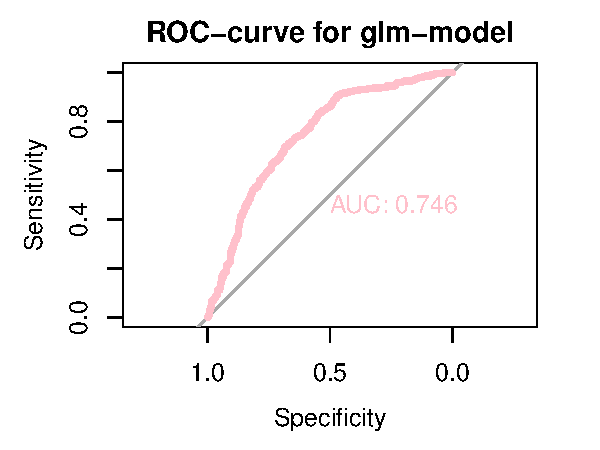
\includegraphics{Exercise1_files/figure-latex/unnamed-chunk-19-1} \end{center}

\begin{Shaded}
\begin{Highlighting}[]
\NormalTok{qda\_roc }\OtherTok{\textless{}{-}} \FunctionTok{roc}\NormalTok{(}\AttributeTok{response =}\NormalTok{ test}\SpecialCharTok{$}\NormalTok{class, }\AttributeTok{predictor =}\NormalTok{ qda\_predicted}\SpecialCharTok{$}\NormalTok{posterior[,}\StringTok{"1"}\NormalTok{])}
\FunctionTok{plot}\NormalTok{(qda\_roc, }\AttributeTok{col=}\StringTok{"purple"}\NormalTok{, }\AttributeTok{lwd=}\DecValTok{4}\NormalTok{, }\AttributeTok{print.auc=}\ConstantTok{TRUE}\NormalTok{, }\AttributeTok{main=}\StringTok{"ROC{-}curve for qda{-}model"}\NormalTok{)}
\end{Highlighting}
\end{Shaded}

\begin{center}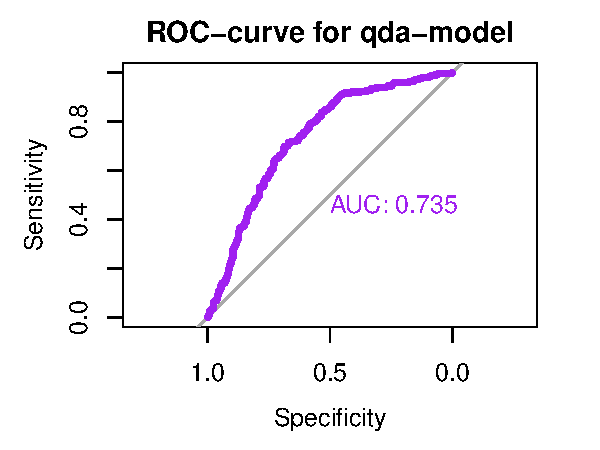
\includegraphics{Exercise1_files/figure-latex/unnamed-chunk-19-2} \end{center}

\begin{Shaded}
\begin{Highlighting}[]
\NormalTok{knn\_probabilities }\OtherTok{\textless{}{-}} \FunctionTok{ifelse}\NormalTok{(knn\_model }\SpecialCharTok{==} \DecValTok{0}\NormalTok{, }\DecValTok{1} \SpecialCharTok{{-}} \FunctionTok{attributes}\NormalTok{(knn\_model)}\SpecialCharTok{$}\NormalTok{prob,}\FunctionTok{attributes}\NormalTok{(knn\_model)}\SpecialCharTok{$}\NormalTok{prob)}
\NormalTok{knn\_roc }\OtherTok{\textless{}{-}} \FunctionTok{roc}\NormalTok{(}\AttributeTok{response =}\NormalTok{ test}\SpecialCharTok{$}\NormalTok{class, }\AttributeTok{predictor =}\NormalTok{ knn\_probabilities)}
\FunctionTok{plot}\NormalTok{(knn\_roc, }\AttributeTok{col=}\StringTok{"turquoise"}\NormalTok{, }\AttributeTok{lwd=}\DecValTok{4}\NormalTok{, }\AttributeTok{print.auc=}\ConstantTok{TRUE}\NormalTok{, }\AttributeTok{main=}\StringTok{"ROC curve knn{-}model"}\NormalTok{)}
\end{Highlighting}
\end{Shaded}

\begin{center}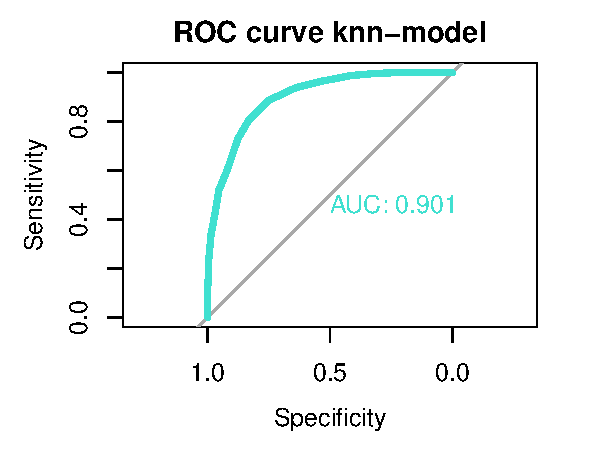
\includegraphics{Exercise1_files/figure-latex/unnamed-chunk-19-3} \end{center}

\hypertarget{iv}{%
\subsubsection{(iv)}\label{iv}}

Glm and QDA performs similar for ROC, while KKN performs significantly
better. Would therefore choose the KNN-classifier for this problem.

\hypertarget{problem-4}{%
\section{Problem 4}\label{problem-4}}

\hypertarget{a-2}{%
\subsection{a)}\label{a-2}}

\hypertarget{b-2}{%
\subsection{b)}\label{b-2}}

(i): False, (ii): False, (iii): True, (iv): False

\end{document}
